\chapter{About Contracts}

Contract Programming, also known as Design by Contract, is a methodology that can be used for software design and development [1]. This chapter gives a brief history and walks through different aspects of it.

\section{History and Background}

Design by Contract methodology was first introduced to the public by Bertrand Meyer as a part of his programming language named Eiffel. Contract Programming is an integral part of Eiffel, but the methodology in itself can be used in any language. Figure.~\ref{fig:EiffelContract} shows an example of how contracts are written in the Eiffel programming language [2].

\begin{figure}[htb]
\centering
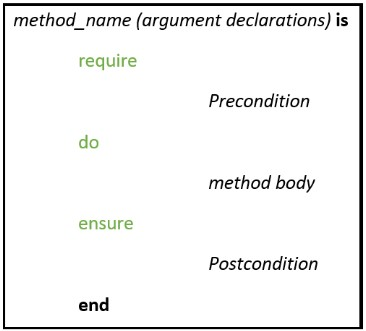
\includegraphics[width=0.5\textwidth]{images/EiffelContract.jpg}
\caption{Contract in Eiffel.} 
\label{fig:EiffelContract}
\end{figure}

Another important aspect of Contract Programming is that it helps build and design a robust and fault tolerant software system, which is why it has been used repeatedly by many developers in the form of libraries or as a language feature.
Contract Programming uses a contract agreed upon by both the developer of the software and the user of the software. In Meyer's terms, a developer is the supplier and a user is the client [1].  
Here the user of the software must agree and abide to the preconditions that contract specifies. If the user has done so, then the method should return the results that satisfy the post-conditions. In this way, when a software system runs into an error state it is very easy for one to detect who is to be blamed. If the problem is with the preconditions, then it is the client who is to be blamed [2]. If the problem is with the results, which means the post-conditions are not met, then the software system has a defect on the side of the supplier. This way it is ensured that the software system does what it is supposed to and that any errors can be easily identified.

\section{Benefits of Design by Contract (DbC)}

Developing a software system using DbC methodology not only makes it more reliable but also has some other added advantages. Using DbC ensures that the software system has a better design, meaningful exceptions, better documentation and easier debugging [3].

\subsection{Better Design}
Careful use of DbC by software developers can yield better designed systems. This is because a relationship between the client and the supplier is more clearly expressed in the form of conditions. While writing method routines programmers have to clearly think about the preconditions and post-conditions that are declared. This ensures that the system being developed adheres to all the functional specifications. It also makes programmer think about all the exceptional situations that the program may run into while writing the code. This makes it more reliable and at the same time helps to achieve a clearer design.

\subsection{Meaningful Exceptions}
In the case of DbC, a program runs into an exception only when it fails the contract. As a result, it is very easy to identify the exact cause behind its occurrence. For example, if the exception occurred because of a failed precondition then the cause is that some inconsistent or bad input values were passed to the method routine. This helps the programmer develop clear and meaningful exceptions that can be easily understood by the client.
Figure.~\ref{fig:FailedContract} shows an example of an exception thrown as a result of a failed contract. 
\linebreak
\linebreak
\begin{figure}[htb]
\centering
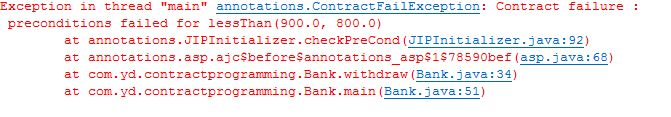
\includegraphics[width=1.0\textwidth]{images/ContractFailedException.PNG}
\caption{Exception on Failed Contract.} 
\label{fig:FailedContract}
\end{figure}

\subsection{Better Documentation}
Contracts defined for the system by the developer are part of the code that is visible to the client. Client can read through the contracts that are defined by the supplier for the system, forming an easy means of documentation. Also, it may happen that the user made some modifications to the code but failed to update the document. However, since contracts are an integral part of the code that change if the associated code logic has changed, they form consistent form of documentation. Also, contracts provide specific and precise information about the method or routine that they are attached to.

\section{Limitations of Contracts}
Although using contracts adds a little cost (time) to the development process and processing time, it is an overhead. This cost includes, cost of writing contract rules (in this case writing Prolog rules) and cost of executing those contracts at run time for validation checking. These overheads should be considered while making a decision of whether to use DbC methodology in the development process.

\subsection{Cost of Writing Contract Rules}
Developers will have to invest additional time towards writing contracts along with the overall code writing time. Some developers might neglect this work, which can ultimately result into the poor quality contracts [1].
Also, developers need to think about and invest time in writing contracts in the early phases of the software development process, which many developers might think of as an unnecessary task.

\subsection{Contract writing Skills}
Writing good contracts is a skill [1]. For developers who are not used to DbC, learning to write contracts might prove to be a time consuming process. It might be a very difficult task to find experienced developers who already know about writing contracts as it is not a commonly followed practice. Developers will have to invest some extra time initially to learn and understand the skill of writing well designed contract rules.

\subsection{False Sense of Security}
Using contracts increases code reliability, but it does not make them perfect. It can improve the overall quality of the code, but developers should not assume that their code is free of bugs simply because all of the contracts hold true.
